\documentclass[preview]{standalone}

\usepackage{amsmath}
\usepackage{amssymb}
\usepackage{stellar}

\hypersetup{
    colorlinks=true,
    linkcolor=black,
    urlcolor=blue,
    pdftitle={Stellar},
    pdfpagemode=FullScreen,
}

\begin{document}

\title{Stellar}
\id{storia-ottocento}
\genpage

\begin{snippetdefinition}{restaurazione-definizione}{Restaurazione}
    Periodo della storia europea che va dalla fine del regime napoleonico
    all'abdicazione del re di Francia Carlo X di Borbone.
\end{snippetdefinition}

\begin{snippetdefinition}{santa-alleanza-definizione}{Santa alleanza}
    La \textit{Santa alleanza} è stata una coalizione tra le grandi potenze monarchiche della Russia, dell'Austria e della Prussia.
    La Santa Alleanza fu creata dopo la sconfitta di Napoleone.
\end{snippetdefinition}

\section{Liberalismo}

\begin{snippet}{movimento-liberale-conservatore}
    Principalmente possiamo distinguere il \textit{movimento liberale} (non ancora \textbf{partito})
    e il \textit{movimento conservatore}.

    Il liberalismo è caratterizzato dalle seguenti proprietà:
    \begin{itemize}
        \item Fiducia nell'individuo.
        \item Libertà individuo di fronte allo Stato.
        \item Libertà dell'individuo devono essere garantite.
        \item Aspirazioni della ricca borghesia.
        \item Libertà e uguaglianza \(\rightarrow\) entrano in conflitto.
        \item Movimento democratico-liberale \(\rightarrow\) uguaglianza.
        \item Sovranità popolare \(\rightarrow\) individuo partecipa alle attività dello Stato.
    \end{itemize}

    Il movimento liberale ha origini in realtà nel 1700 perché si oppone
    all'assolutismo monarchico, assolutismo che tornerà nel 1800 con la restaurazione.
    Ha le sue radici nelle idee dell'illuminismo e nei principi di libertà individuale e di autodeterminazione.

    Viene rimpiazzata la monarchia costituzionale con il parlamento eletto (suffragio censitario)
    \(\rightarrow\) sovranità nazionale.
    Il potere dello Stato deve essere limitato e favorire la libertà d'azione.
\end{snippet}

\section{Liberalismo moderato o conversatore}

\begin{snippet}{liberalismo-moderato-conservatore}
    \textbf{Libertà da:}
    \begin{itemize}
        \item \textbf{Libertà dallo Stato:} Questo concetto è legato alla cosiddetta libertà negativa, che si riferisce alla protezione dell'individuo
            dall'interferenza o coercizione dello Stato o di altri individui.
            Nel contesto storico menzionato nel documento, questo concetto è particolarmente
            rilevante durante il secolo XVIII, un periodo in cui si iniziava
            a chiedere un minor intervento dello Stato nella vita delle persone.
    \end{itemize}

    \textbf{Libertà di:}
    \begin{itemize}
        % di partecipare alla vita politica
        \item \textbf{Libertà di parola, riunione, associazione:} Questi sono diritti fondamentali che il liberalismo sostiene debbano essere protetti da qualsiasi forma di oppressione o limitazione.
        \item \textbf{Libertà di stampa, culto, attività economica:} Allo stesso modo, queste libertà sono viste come essenziali per il pieno sviluppo e la realizzazione dell'individuo.
        \item \textbf{Diritto inviolabile della proprietà:} Questo è un pilastro fondamentale del pensiero liberale, che vede la proprietà privata come un diritto sacro e inviolabile.
    \end{itemize}

    Il ceto sociale di riferimento è la borghesia, per cui il sistema è verticista e censitario (solo chi
    ha le capacità, il tempo ed è proprietario o contribuisce alla ricchezza dello Stato può governare
    ed è in grado di farlo).
    Si mira a favorire in primo luogo lo sviluppo economico e di riflesso anche la stabilità sociale.

    \begin{itemize}
        \item Più lo stato è limitato, più l'uomo è libero di agire (in contrapposizione con l'assolutismo).
        \item Libertà sì, ma con moderazione, libertà di voto ma non per tutti (solo possedenti). Realizzazione graduale dell'assetto del liberalismo, possono scendere a compromessi con l'antico regime.
    \end{itemize}
\end{snippet}

\section{Liberalismo radicale o democratico}

\begin{snippet}{0216d89a-c1b6-4a2f-86a3-179211a380c4}
    In generale si riprendono i prinipi del liberlismo, ma in modo più radicale.
    Invece ad una monarchia parlamentare, preferiscono una repubblica con un sistema rappresentativo (suffragio universale).

    \begin{itemize}
        \item L'uomo è tanto più libero se può esercitare le prorpie libertà, se non è limitato o escluso dalla povertà o dalla malattia, chi lo è non ha i mezzi per poter godere delle proprie libertà.
        \item Trasformazione rapida della società, cambiamento deciso; volontà di stravolgere la società di antico regime. Vogliono coinvolgere tutta la popolazione (democratici): referendum, suffragio universale.
    \end{itemize}

    Il liberalismo radicale presta maggiore attenzione ai ceti popolari e mira a coniugare sviluppo
    economico e stabilità sociale. La corrente radicale, che promuove in modo particolare
    l'uguaglianza economica e sociale si avvicina al pensiero socialista (senza però l'abolizione della
    proprietà privata).
\end{snippet}

\section{Pensiero conservatore}

\begin{snippetdefinition}{conservatorismo-definizione}{Conservatorismo}
    Con \textit{conservatorismo} si intende l'insieme delle ideologie che, variamente, si oppongono al progresso. Il
    concetto di conservatorismo appartiene esclusivamente al lessico politico moderno.
\end{snippetdefinition}

\begin{snippet}{e8db34f7-16f9-4209-8a8b-87066cc41f8f}
    Il partito conservatore fra il '700 e '800 si opponeva all'illuminismo e a tutto ciò che portava la Rivoluzione Francese.
    Il pensiero conservatore è l'antitesi del liberalismo.

    Si oppone originariamente al concetto di eguaglianza fra gli umani. Secondo loro, le differenze fra gli uomi sono naturali.
\end{snippet}

\section{Schema riassuntivo}

\begin{snippet}{ddef50ba-3d76-4965-8fe3-30d9f2b86091}
    \begin{enumerate}
        \item \textbf{Risoluzionari}: Cambiamento radicale forzato uso della violenza.
        \item \textbf{Progressisti}: Cambiamento graduale tramite riforme.
        \item \textbf{Conservatori}: Rispetto della tradizione, mutare il presente nel rispetto della tradizionare.
        \item \textbf{Reazionari}: Vogliono ritornare ad un regime precedente.
    \end{enumerate}
    
    \textbf{Conservatori:}
    \begin{itemize}
        \item Monarchia assoluta.
        \item Rafforzamento delle gerarchie di potere (clero e nobiltà).
        \item Difesa della tradizione.
        \item Potere per diritto divino, nessuna rappresentanza popolare.
    \end{itemize}
    
    \textbf{Liberali:}
    \begin{itemize}
        \item Monarchia costituzionale.
        \item Rispetto dell'autonomia dell'individuo e della ragione.
        \item Idea di progresso
        \item Potere delle èlite borghesi, che devono essere rappresentate.
    \end{itemize}
\end{snippet}

\section{Socialismo}

\begin{snippet}{socialismo-nascita-expl}
    A partire dagli anni Venti dell'Ottocento, i termini socialismo e socialisti vennero usati per
    definire l'atteggiamento critico assunto, da numerosi intellettuali, nei confronti dei
    problemi provocati dal processo di industrializzazione. Più esattamente, le due espressioni
    appena citate furono impiegate per indicare la posizione di coloro che, come rimedio alle
    drammatiche condizioni degli operai e alla diseguaglianza sociale, proponevano la
    soppressione della proprietà privata e la tutela delle classi dei lavoratori.

    \begin{enumerate}
        \item Con la rivoluzione industriale;
        \item muta in modo drastico la vita di milioni di essere umani;
        \item radicale cambiamento nel sistema di produzione;
        \item massiccio impiego di donne e bembini;
        \item sorgono, nelle città, quartieri operai privi di servizi elementari;
        \item trasformazione del mondo agricolo a quello industriale, con conseguenze mutamento della società e l'emergere di nuove classi sociali (borghesia / proletariato).
    \end{enumerate}
    
    I primi sindacati furono le \textit{Trade Unions} in Inghilterra, occupandosi si salvaguardare il proletariato.
\end{snippet}

\begin{snippetdefinition}{socialismo-definizione}{Socialismo}
    Il socialismo, a partire dagli anni Venti dell'Ottocento, rappresentava una reazione critica all'industrializzazione, sostenendo la soppressione della proprietà privata e la protezione dei lavoratori come rimedio alle condizioni drammatiche degli operai e alla disuguaglianza sociale.
\end{snippetdefinition}

\begin{snippet}{tipologia-di-socialismo}
    \textbf{Socialismo utopico}: Le figure chiave del socialismo utopico includono Charles Fourier e Robert Owen.
    Questi pensatori immaginavano comunità ideali basate sulla cooperazione e l'uguaglianza,
    ma spesso mancavano di un piano dettagliato per attuare queste visioni nella pratica.
    Il socialismo utopico è stato successivamente superato dall'approccio più scientifico
    ed economico del socialismo marxista.

    Esistono quindi altri tipologie di socialismo, come quello \textbf{scientifico}.
    Secondo i socialisti, specialmente quelli scientifici, abolire la proprietà privata
    potrebbe portare a qualcosa di nuovo e rinnovato.

    Le idee possono essere riassunte con i seguenti punti:
    \begin{enumerate}
        \item Il socialismo (e successivamente comunismo) va applicato gradualmente. In primis, quando il capitalismo entrerà in contradizione con sè stesso.
        Questa contraddizione deriveré dallo scontro fra borghesia e proletariato.
        \item Lotta di classe, ossia l'idea cje la società umana sia passata attraverso 4 fasi
        (comunità primitive, regime di schiavitù, società feudale, società borghese).
        Per cui l'intera società è costituita da uno scontro fra gli oppressori ed oppressi.
        \item Tutto, fra cui i pensieri, scaturisca dal materialismo e dai bisogni umani.
        Divisione fra \textbf{struttura} (modi di produzione della ricchezza)
        e \textbf{sovrastruttura} (politica, arte, religione, etc).
        Dai modi di produrre ricchezza, si sviluppana la società con le sue idee.
        Se non ci sono classi sociali non ci possono essere lotte di classe.
    \end{enumerate}
\end{snippet}

\begin{snippet}{falansterio-illustration}
    \begin{center}
    \begin{figure}[h]
        \centering
        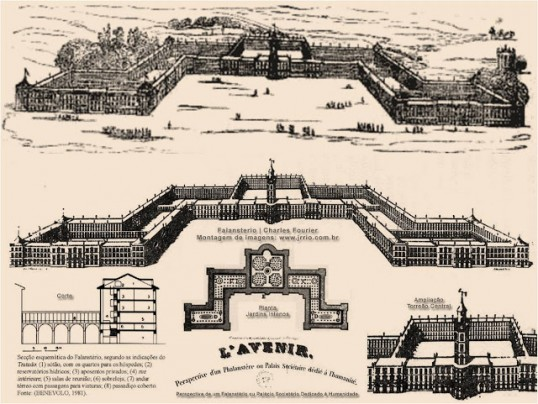
\includegraphics[width=0.75\textwidth]{./resources/falansterio.jpg}
    \end{figure}
    \end{center}
\end{snippet}

\begin{snippet}{cee5a06e-e888-4d1b-aa45-a095ac507beb}
    Secono il testo di Marx, la vittoria è quando abbiamo una massima unità del proletariato.
    Per ottenere il dominio sulla classe borghese è necessario accumulare ricchezza e capitale.
    Questo ricchezza va ottenuta mente il lavoro salariato, il quale fonda concorrenza fra operai.
    Ciò porta al progresso dell'industria ma sostiuisce l'isolamento degli operai con associazione degli operati (unione del proletariato).

    Nonostante viene ritenuto che questa rivoluzione sarebbe prima o poi avvenuta, gli operai e il proletariato,
    pur essendo la maggioranza, non giungono a questa meta.

    Fino al 1970 circa i termini marxismo e leninismo sono praticamente sinonimi.
    Rimangono comunisti tutti coloro che ritengo che la lotta di classe sia inevitabile.
\end{snippet}

\section{Nazione, Nazionalità, Nazionalismo}

\begin{snippetdefinition}{nazione-definizione}{Nazione}
    Nel medioevo, \textit{nazione} aveva un significato puramente geografico.
    Ma dagli inizi dell'Ottocento, nel clima del Romanticismo, il
    termine nazione si carica di un nuovo significato e indica una individualità storica, una
    comunità umana, un popolo che si differenzia da altri popoli sulla base delle sue
    caratteristiche: il profilo etnico o la consanguineità, il legame con un territorio, la lingua, la
    cultura, le esperienze storiche, le consuetudini che regolano la vita comune, le tradizioni
    civili e religiose.
\end{snippetdefinition}

\begin{snippet}{differenza-concetto-di-nazione}
    Quando consideriamo un fattore etnico abbiamo il \textit{concetto naturalistico},
    entre quando parliamo di stare assieme sulla base di esperienze comuni, abbiamo il \textit{concetto volontaristico}.
    Quest'ultimo concetto ci dice che la nazione è un prodotto culturale.

    \textbf{Renan: Cos'è una nazione (concetto volontaristico)}
    \begin{itemize}
        \item Caratteristice legate alla cultura, alla storia;
        \item condivisione di cultura, modo di fare;
        \item eredità di ricordi e consenso attuale \(\rightarrow\) eredi di un patrimonio;
        \item è una scelta.
        \item Prima nasce lo Stato, poi la Nazione.
    \end{itemize}

    \textbf{Fichte: Cos'è una nazione (concetto naturalistico)}
    \begin{itemize}
        \item Stirpe/origini/lingua/territoria;
        \item lingua \(\rightarrow\) recupero dell'identità originaria della nazione;
        \item non è una scelta.
        \item Prima nasce la Nazione, poi lo Stato.
    \end{itemize}

    \textbf{Concetto volontaristico:}
    \begin{itemize}
        \item Sentimento di identità e spinta a stare assieme sulla base di esperienze comuni.
        \item Nazione come prodotto culturale in cui si valorizzano gli aspetti storici e ideali che connotano un popolo.
        \item Idea di poter scegliere.
        \item Concetto volontaristico, volontà di condividere principi, valori, comune sentire.
        \item Illuminismo e riv. Francese come radici culturali di questo concetto (concezione francese).
    \end{itemize}

    \textbf{Concetto naturalistico:}
    \begin{itemize}
        \item Fattori etnici: la nazione è un fattore naturale, oggettivo, basato su elementi come l'etnia, il territorio (lingua, letteratura, tradizioni culturali).
        \item L'appartenenza nazionale di una persona è predestinata (non si può scegliere).
        \item Romanticismo e Restaurazione ne sono il contesto (concezione tedesca).
    \end{itemize}
\end{snippet}

\end{document}